\documentclass[a4paper,man,biblatex]{apa6}
\usepackage[american]{babel}
\usepackage{csquotes}
\usepackage[backend=biber]{biblatex}
\usepackage[document]{ragged2e}
\setlength{\RaggedRightParindent}{0.5in}
\addbibresource{references.bib}
\usepackage{graphicx}
\usepackage{url}
\usepackage{xpatch}
\xpatchbibdriver{online}
  {\printfield{entrysubtype}}
  {\printfield{entrysubtype}%
   \newunit\newblock
   \printfield{note}}
  {}
  {}

\renewcommand{\abstract}[1]{}

\title{The Rankability of Data}
\shorttitle{The Rankability of Data}
\author{Armant Touche}
\affiliation{Portland State University}
\date{\today}

\begin{document}
\thispagestyle{otherpage}
\setcounter{biburllcpenalty}{7000}
\setcounter{biburlucpenalty}{8000}

%\maketitle

\noindent Name: Armant Touche\newline
\noindent Date: 4/29/2020

\subsection{Description} I wanted to share an article on something I remembered hearing when I was in high school around 2010. On the news, I remembered hearing that our global oil reserve were predicted to be depleted by 2030 and have a peak around 2020. Marion King Hubbert in 1956 was scientist who worked at Shell lab and during his tenure there, he created the "Hubbert Curve" which predicted that oil depletion occur around 2000. His ideas were mostly forgotten and were updated by two scientists in the 1980s which suggested the oil peak in global reserves would be peak between 2004-2005. Reduction in global of liquid hasn't occurred.  Apparently there is a lot to the oil industry being there are classifications to oil. One classification being "conventional" and the other being "non-conventional." Crude oil is considered conventional oil. The common metric being used to help predict these peaks is a million barrels used per day (Mb/d). Around 2010, the maximum value for oil usage was close to 75 Mb/d. The prediction was almost correct but was a off by a couple of years but the updated study from 1998 was correct in predicting that peak oil usage would occur in the near future. Still, oil peak included both conventional and non-conventional which is an important distinction. Oil peak metric only applied to (flowable) oil and since non-conventional oil does not normally need to be "discovered." The takeaway was that there was a gap in data when it came to measuring oil discoveries and oil usage. They study wasn't wrong in predicting the oil usage peak that occurred around 2010. Unfortunately, article I am sharing states that comparing absolutes are incompatible with mainstream views economic system.

            \begin{center}
            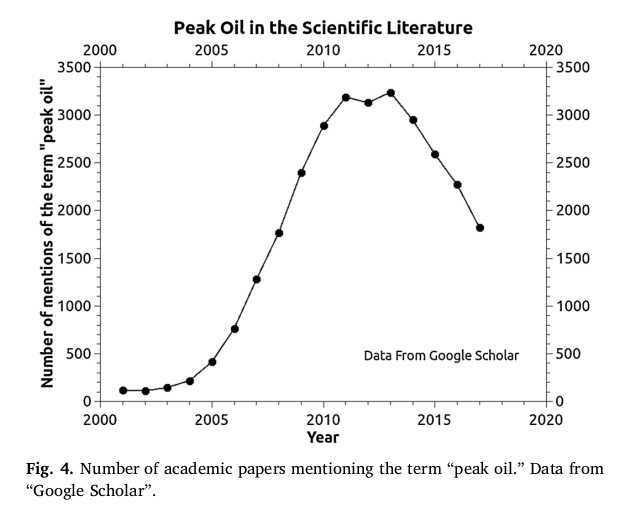
\includegraphics[width=.5\textwidth]{google_data}
            \end{center}

\subsection{Why} The reason I think this study is important is because big a prediction like the one I am sharing deserve more studies because conventional oil powers a lot of economies. From the same study, the are subtler elements that needed to be study. One element being that predictive models are often pessimistic which can cause a decline in research interest. Research keyword data from Google's Scholar application graphed "oil peak" usage in scientific literature and since 2013, the lack of mentioning "oil peak" declined from a peak of around 3250 mentions per year to 1750 mentions per year. The decline in mentions highlight the decline in interest which is unfortunate. One of reasons the author of the study suggested for the decline in interest was that the peak oil idea clashed with mainstream views and that it was a minority opinion. Hopefully with new data, better prediction could be made in reference to global oil reserves because the constant need for output has to stop increasing anytime in the future. When that time will come, well, data is needed to make that prediction.

\printbibliography

\end{document}
